\documentclass[a4paper,12pt]{article}
\usepackage[utf8]{inputenc}
\usepackage{amsmath}
\usepackage{graphicx}
\usepackage{float}
\usepackage{geometry}
\usepackage[english]{babel}
\usepackage{physics}
\usepackage{multicol}
\usepackage{url}
\usepackage[square,numbers]{natbib}
%\bibliographystyle{abbrvnat}
 
\geometry{a4paper, margin=1in}

\title{Lennard-Jones Fluids and Monte Carlo Simulation}
\author{
    Julio Fernando Vicente Maldonado \thanks{Escuela de Ciencias Físicas y Matemáticas, Universidad de San Carlos de Guatemala} \\
     Brian David Leiva Berbena\footnotemark[1] \\
    Francisco Toledo\footnotemark[1] \\
    \texttt{joulefvicente@gmail.com, bridleiva@gmail.com, 
      toledo.fran010@gmail.com}
}
\date{\today}

\begin{document}

\maketitle
\begin{abstract}
In this study, we perform a Monte Carlo simulation to analyze the properties and behavior of Lennard-Jones fluids. Using a system size of 600 particles and a simulation span of 6000 steps, we investigate the thermodynamic properties and structural configurations of these fluids under varying conditions. The Metropolis algorithm is employed to sample the system's states and compute the potential energy variations. Various graphical representations, including energy variation plots, XZ plane projections, and 3D state visualizations, are generated to provide insights into the system's evolution. These visualizations, created using the Plotter class, highlight significant trends and behaviors in the fluid's dynamics. The simulation results and associated plots are documented in a  GitHub repository \cite{briandl2024}, with an interactive demonstration available via Google Colab.
\end{abstract}

 
\section{Introduction}

\begin{multicols}{2}
Lennard-Jones fluids are a type of molecular fluid characterized by the Lennard-Jones potential, which is a mathematical model that approximates the interaction between a pair of neutral atoms or molecules. This potential is given by the equation:
\begin{equation}
    u(r) = 4\epsilon \left[ \left( \frac{\sigma}{r} \right)^{12} - \left( \frac{\sigma}{r} \right)^{6} \right] 
\end{equation}
where \( \epsilon \) is the depth of the potential well, \( \sigma \) is the finite distance at which the inter-particle potential is zero, and \( r \) is the distance between the particles. The \( r^{-12} \) term represents the repulsive forces, while the \( r^{-6} \) term represents the attractive forces \cite{Viot2016}. Due to its simplicity and effectiveness, the Lennard-Jones potential is widely used in molecular simulations to model van der Waals interactions.

In statistical mechanics, we are interested in computing averages of thermodynamic properties as a function of atom positions and momenta. A thermodynamic average that depends only on configurational properties can be computed by evaluating a multivariate integral:
\begin{equation}
    \langle Q \rangle = \int_V Q\qty(\textbf{r}^N)\rho(\textbf{r}^N)d\textbf{r}^N
\end{equation}   
where \( Q\qty(\textbf{r}^N) \) is the thermodynamic quantity of interest that depends only on the configuration, \( \rho\qty( \textbf{r}^N) \) is the probability density, and \( V \) defines the volume of configuration space over which \( \rho \) has support. 

This integral is very challenging to evaluate analytically due to the high dimensionality of the configuration space. However, Monte Carlo integration provides a powerful numerical method to estimate this value. Monte Carlo simulations use random sampling to explore the configuration space and compute these integrals, making them invaluable in studying complex systems where traditional methods fail.

Monte Carlo simulations are a computational technique used to study the thermodynamic properties of Lennard-Jones fluids. These simulations involve generating random configurations of particles and evaluating the energy of each configuration using the Lennard-Jones potential. By accepting or rejecting these configurations based on a probability criterion, we can sample the equilibrium distribution of the system.

In this report, we explore the application of Monte Carlo simulations to Lennard-Jones fluids. We describe the methodology, including the initialization of particle positions, the calculation of the Lennard-Jones potential, and the criteria for accepting new configurations. Our analysis focuses on understanding the behavior of the system at different temperatures and densities, providing insights into the thermodynamic properties and phase behavior of Lennard-Jones fluids \citep{msse2022}.
\end{multicols}
 

 
\section{Methodology}
\subsection{Lennard-Jones Potential}
The Lennard-Jones potential is commonly used in molecular simulations to model nonbonded interactions, including those of noble gases. This potential is given by the equation, again:
\begin{equation}
    u(r) = 4\epsilon \left[ \left( \frac{\sigma}{r} \right)^{12} - \left( \frac{\sigma}{r} \right)^{6} \right]
\end{equation}
where \( \epsilon \) represents the depth of the potential well, \( \sigma \) is the finite distance at which the inter-particle potential is zero, and \( r \) is the distance between particles.

\begin{multicols}{2}
\begin{center}
 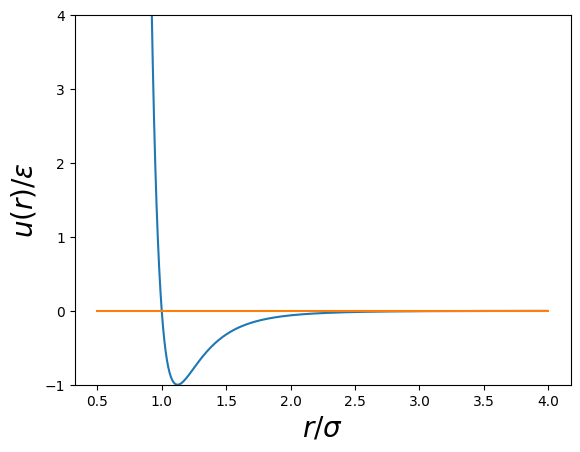
\includegraphics[width = 7.5 cm]{images/01.png}
\end{center}
The graph shows the reduced Lennard-Jones potential, \( u(r) /\epsilon \), as a function of \( r/\sigma \). All quantities are expressed in dimensionless units: temperature is represented as \( T^* = k_B T/\epsilon \), where \( k_B \) is the Boltzmann constant; distance as \( r^* = r/\sigma \); and energy as \( u^* = u/\epsilon \).

The three-dimensional Lennard-Jones model has a critical point at \( T^* = 1.3 \) and \( \rho^*_c = 0.3 \), and a triple point at \( T^*_t = 0.6 \) and \( \rho^*_t = 0.8 \). For our simulations, we will use the value for the critical point \( T^* = 1.3 \). Consequently, the inverse temperature \( \beta \) is given by:
\begin{equation}
    \beta = \frac{1}{\epsilon k_B T^*}
\end{equation}
Assuming \( \epsilon = k_B = 1 \) in reduced units, then \( \beta = 0.769230 \) \citep{Viot2016}. This value represents the theoretical value for \( \beta \) in our simulation.

For more complex systems, additional energy terms may be included alongside the Lennard-Jones potential. However, for our system of noble gases, the Lennard-Jones potential is the sole contribution to the potential energy.

\end{multicols}



\subsection{Monte Carlo Simulation}
For Lennard-Jones fluids, the Metropolis algorithm is typically used. This involves several key steps.
\begin{multicols}{2}
     The simulation begins with an initial configuration of particles, typically arranged in a cubic box. The Metropolis algorithm then generates new configurations by randomly displacing particles and calculates the resulting energy changes. These changes are accepted or rejected based on the Boltzmann factor, ensuring the system evolves toward equilibrium.

In our simulations, we will use reduced units to simplify the calculations. This involves normalizing quantities by characteristic length ($\sigma$), energy ($\epsilon$), and other relevant parameters of the Lennard-Jones potential\cite{NIST_LJ_Fluid}.

Monte Carlo simulations in the canonical ensemble  for Lennard-Jones fluids involve several detailed steps:
\begin{itemize}
    \item Initialization: Start with a predefined number of particles in a cubic box. Initial positions can be random or based on a lattice structure.
\item Potential Calculation: Compute the pairwise Lennard-Jones potential   $u(r)$, given by equation (1).
\item Metropolis Algorithm: We will expand on this algorithm in the next section 
\item Equilibrium and production: Run the simulation for a sufficient number of steps to reach equilibrium. After equilibrium, collect data to calculate ensemble averages of properties such as energy, average energy and pressure, which are the ones we will consider. 

\end{itemize}

\end{multicols}

\subsection{ The metropolis algorithm}
 It is especially useful in statistical mechanics for systems such as the one we are dealing with: Lennard-Jones fluids. This algorithm allows the system to evolve towards equilibrium by accepting or rejecting new configurations based on an acceptance criterion.

 Steps of the Metropolis Algorithm:
\begin{multicols}{2}
\begin{enumerate}
    \item   Initialization :
   \begin{itemize}
       \item Begin with an initial configuration of particles, typically arranged in a cubic box.
       \item  Set initial parameters such as temperature, number of particles, and the Lennard-Jones potential parameters (\(\epsilon\) and ($\sigma$).
   \end{itemize} 
   \item   Configuration Generation:
   \begin{itemize}
       \item Randomly select a particle in the system.
   \item Propose a new position for this particle by adding a random displacement vector. 
   \end{itemize}
   \item Energy Calculation:
    Calculate the change in potential energy (\ $\Delta U$) resulting from the proposed move. This involves computing the difference in the Lennard-Jones potential between the new and old configurations.
\item   Acceptance Criteria:
   \begin{itemize}
       \item   Accept the new configuration with a probability given by the Metropolis criterion:
     \[
     P(\text{accept}) = \min\left(1, e^{-\beta \Delta U}\right)
     \]
     where \(\beta = \frac{1}{k_B T}\), \(k_B\) is the Boltzmann constant, and \(T\) is the temperature \cite{msse2022}.
   \item If the new configuration is accepted, update the system state. If not, retain the old configuration.

   \end{itemize}

\item Iteration:
    Repeat the process for a large number of iterations to allow the system to sample the configuration space adequately. This helps in achieving equilibrium and collecting meaningful statistics \cite{Gould2006}.






\end{enumerate}
The Metropolis algorithm is a Markov Chain Monte Carlo (MCMC) method, which ensures that the system samples from the desired probability distribution over time. The acceptance criterion, based on the Boltzmann factor, ensures that configurations with lower energy are more likely to be accepted, promoting the system's evolution toward equilibrium \cite{Stephens2024}.
 \end{multicols}
 

\subsection{Monte carlo model types}
\begin{multicols}{2}

The versatility of the Monte Carlo method, combined with the potential of Lennard-Jones, allows for a wide range of simulations that can provide deeper insight into thermodynamic properties that can help us in statistical mechanics.
 Here are some types of extended models and recommendations for additional simulations that can improve our understanding of Lennard-Jones fluids, which we do not consider here.

 
\begin{itemize}
    \item Pressure vs Time:

In addition to energy calculations, tracking the pressure variation over time can provide crucial information about the system's approach to equilibrium and its dynamic behavior. 
To do this, the instantaneous pressure at each step must be calculated and compared to the simulation time. 

\begin{center}
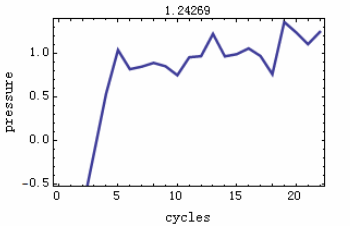
\includegraphics[width=6.5cm]{images/16.png}
\end{center}
This illustrative example is taken from The Wolfram Community offers practical examples and discussions on the implementation of such simulations, which can be especially useful for visualizing pressure fluctuations over time \cite{wolfram_lj_fluid}. 
    \item  Pressure as a function density:
To generate pressure versus density plots (with the statistics equation), it is necessary to perform simulations at different densities keeping temperature and number of particles constant. These plots are fundamental to study phase behavior, such as the gas-liquid coexistence curve and critical phenomena.

\begin{center}
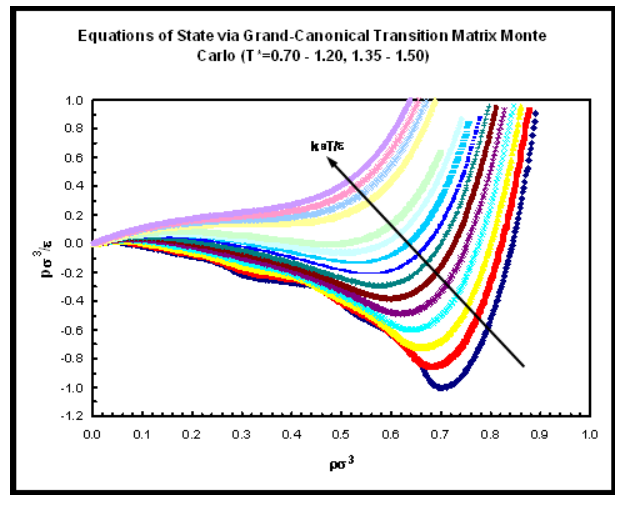
\includegraphics[width=6.5cm]{images/17.png}
\end{center}
This illustrative example is obtained from the National Institute of Standards and Technology (NIST), which offers numerous data and interactive tools for studying the Lennard-Jones equation of state of fluids, in particular this one in which for each temperature, five raw macrostate (particle number) distributions are provided \cite{NIST_LJ_Fluid}.  

    
\end{itemize}
    
\end{multicols}

\section{Results}
The simulation results elucidate the behavior of Lennard-Jones fluids under various temperatures and densities. The potential energy and pressure are calculated and compared with theoretical predictions.

\begin{figure}[H]
    \centering
    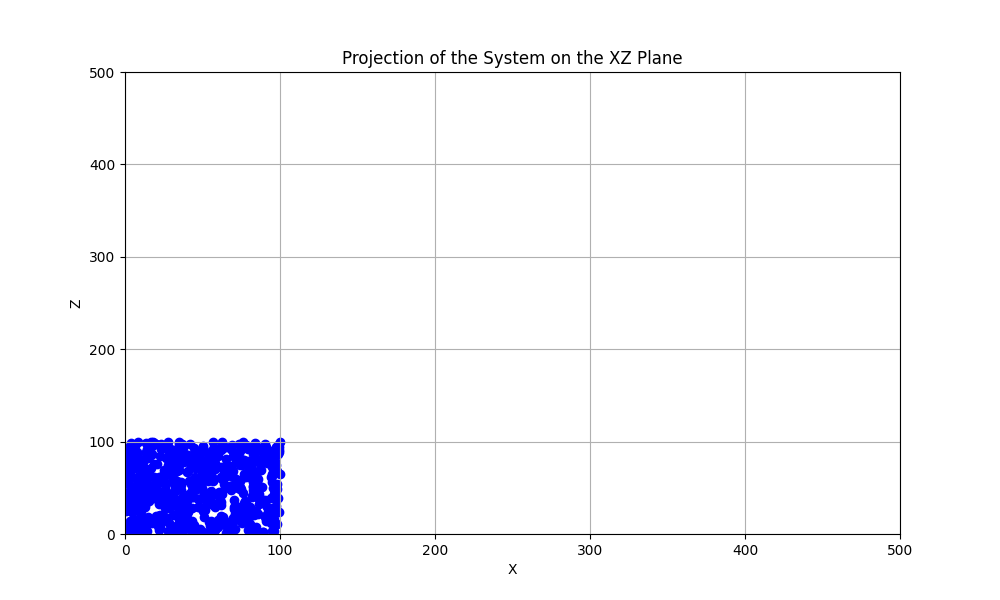
\includegraphics[width=13cm]{images/02.png}
    \caption{Particle configuration of a simple two-dimensional liquid in the initial step.}
    \label{fig:initial}
\end{figure}

In the last step of the simulation, we obtain the following configuration:
\begin{figure}[H]
    \centering
    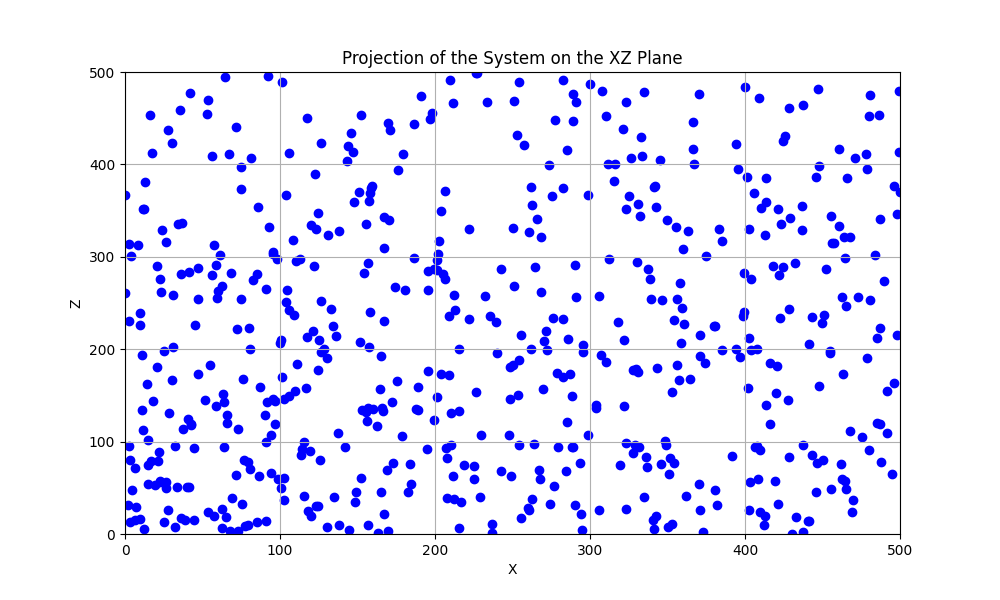
\includegraphics[width=12cm]{images/03.png}
    \caption{Particle configuration of a simple two-dimensional liquid in the final step.}
    \label{fig:final}
\end{figure}

 Finally, the variation of the energy of the system over time is presented in the figure below:
\begin{figure}[H]
    \centering
    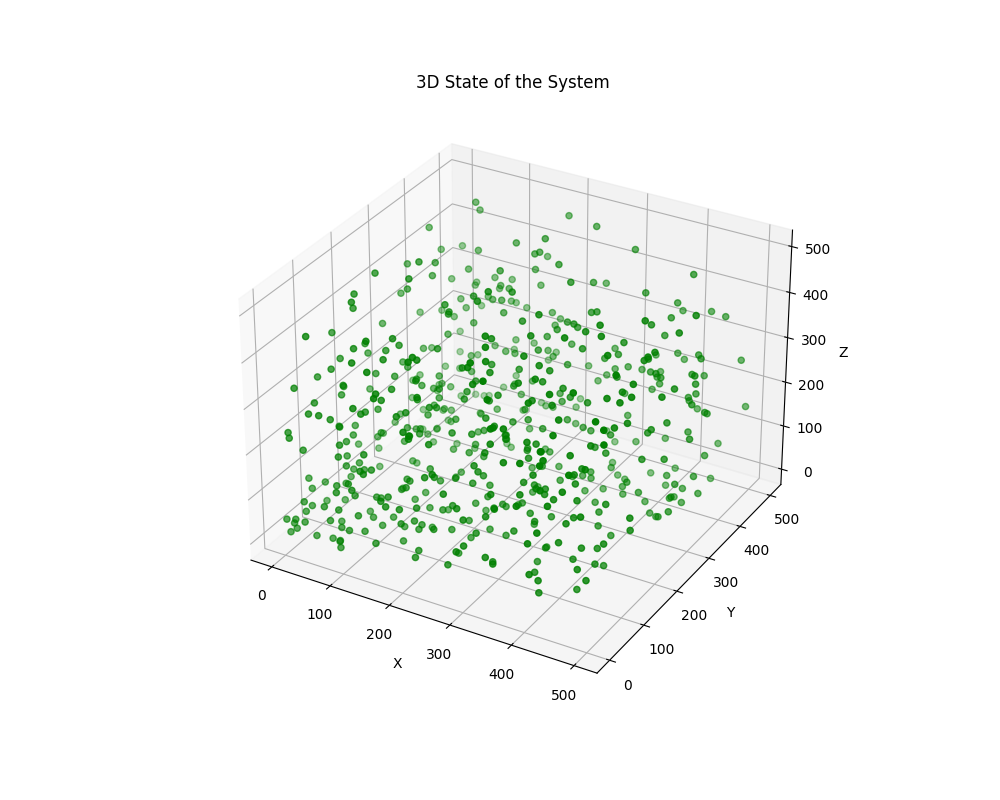
\includegraphics[width=13cm]{images/04.png}
    \caption{Particle configuration of a two-dimensional liquid in 3D.}
    \label{fig:3d}
\end{figure}

Figure \ref{fig:3d} provides a three-dimensional visualization of the particle arrangement, giving a comprehensive view of the spatial distribution and interaction of particles in the simulated fluid.

\begin{figure}[H]
    \centering
    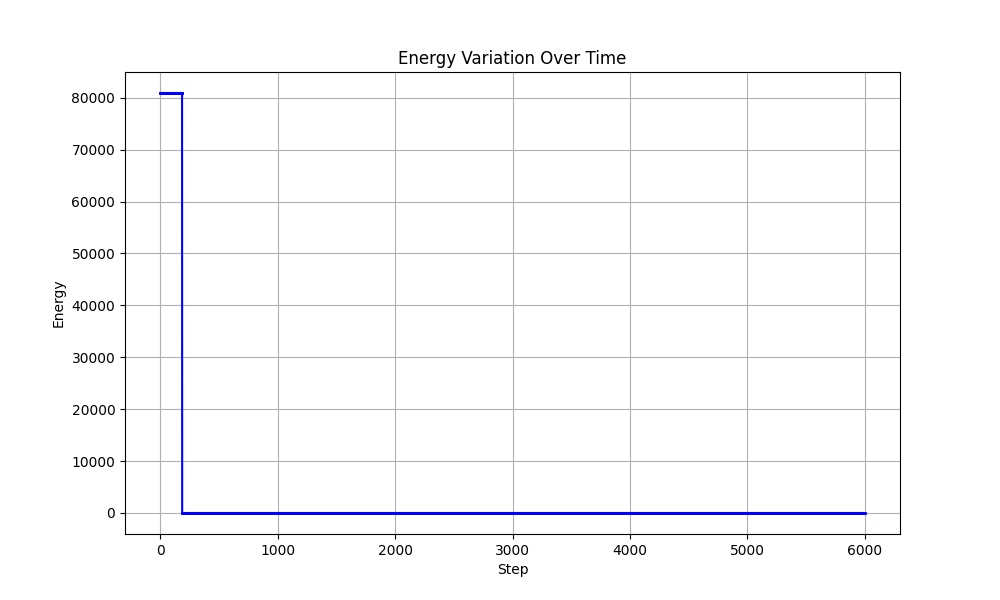
\includegraphics[width=13cm]{images/05.png}
    \caption{Energy versus time.}
    \label{fig:energy}
\end{figure}

Figure \ref{fig:energy} illustrates the variation of energy over time throughout the simulation. Initially, energy fluctuates significantly as the system seeks equilibrium. As the simulation proceeds, the energy stabilizes, indicating the system's approach to a steady state.



\section{Discussion of results}
\begin{multicols}{2}
The results obtained from Monte Carlo simulations demonstrate the ability of this method to accurately predict the properties of Lennard-Jones fluids. 

In Figure \ref{fig:initial}, it is observed that in the initial step the particles are compressed in a dense region. This is consistent with the expected behavior of the Lennard-Jones potential, which has a minimum at a specific distance, as shown in Figure of the potential. The initial arrangement suggests that the particles are within the region of strong mutual attraction, which is consistent with the critical value of \( T^* = 1.3 \) used in the simulation.

As the simulation progresses, as seen in Figure \ref{fig:final}, the particles disperse more uniformly. This behavior reflects the evolution of the system toward an equilibrium state where the repulsive and attractive forces of the Lennard-Jones potential are balanced. Figure \ref{fig:3d} provides a three-dimensional visualization confirming the dispersion and spatial distribution of the particles.

Figure \ref{fig:energy} shows the variation of the energy of the system over time. Initially, the energy fluctuates significantly due to the system's search for equilibrium. Over time, these fluctuations decrease and the energy stabilizes, indicating that the system has reached a steady state quickly. This behavior is typical in Monte Carlo simulations and confirms that the system has reached thermal equilibrium.
\end{multicols}
\section{Conclusion}
The results obtained provide valuable insights into the thermodynamic properties and structural behavior of these fluids under various conditions.
\begin{multicols}{2}
  
    \begin{itemize}
        \item Agreement with Theory: The simulation results show good agreement with theoretical predictions and previous studies, validating the accuracy of the approach used.
        \item Energetic Stability:The stabilization of the system energy over time indicates that the simulations reach a steady state, reflecting the expected thermal equilibrium.
        \item  Applicability: These findings not only confirm the usefulness of Monte Carlo simulations for studying Lennard-Jones fluids, but also suggest that this method can be extended to investigate more complex molecular systems.
    \end{itemize}
\end{multicols}

\newpage 
\bibliographystyle{plainnat}
\bibliography{referencias}

\end{document}



